%%%%%%%%%%%%%%%%%%%%%%%%%%
%%% author : Yamada. T %%%
%%% made for TH series %%%
%%%%%%%%%%%%%%%%%%%%%%%%%%

\documentclass[b5paper,10pt,fleqn] {ltjsarticle}

\usepackage[margin=10truemm]{geometry}

\usepackage{pict2e, graphicx}
\usepackage{tikz}
\usetikzlibrary{intersections,calc,arrows.meta}

\usepackage{amsmath, amssymb, amsthm}
\usepackage{ascmac}
\usepackage{comment}
\usepackage{empheq}
\usepackage[shortlabels,inline]{enumitem}
\usepackage{fancybox}
\usepackage{fancyhdr}
\usepackage{here}
\usepackage{lastpage}
\usepackage{listings, jvlisting}
\usepackage{fixdif}

\usepackage{stmaryrd}
\usepackage[listings]{tcolorbox}
%\usepackage{ascolorbox}
\usepackage{titlesec}
\usepackage{ulem}
\usepackage{url}
\usepackage{verbatim}
\usepackage{wrapfig}
\usepackage{xcolor}
\usepackage{luatexja-ruby}
\usepackage{varwidth}
\usepackage[version=3]{mhchem}
\usepackage{wrapfig}


\usepackage{physics2}
	\usephysicsmodule{ab}
	\usephysicsmodule{ab.braket}
	\usephysicsmodule{ab.legacy}
	%\usephysicsmodule{braket}
	\usephysicsmodule{diagmat}
	\usephysicsmodule{xmat}
	\usephysicsmodule{nabla.legacy}
	\usephysicsmodule{qtext.legacy}

\usepackage[ISO]{diffcoeff}
\difdef { f, s } { D }
{ op-symbol = \mathrm{D} }


\newcommand{\mctext}[1]{\mbox{\textcircled{\scriptsize{#1}}}}
\newcommand{\ctext}[1]{\textcircled{\scriptsize{#1}}}
\newcommand{\ds}{\displaystyle}
\newcommand{\comb}[2]{{}_{#1}\mathrm{C}_{#2}}
\newcommand{\hs}{\hspace}
\newcommand{\vs}{\vspace}
\newcommand{\emphvs}{\vspace{1em}\notag\\}
\newcommand{\ora}{\overrightarrow}
\newcommand{\ol}{\overline}
\newcommand{\oramr}[1]{\overrightarrow{\mathrm{#1}}}
\newcommand{\tri}{\triangle}
\newcommand{\mr}{\mathrm}
\newcommand{\mb}{\mathbb}
\newcommand{\mrvec}[1]{\overrightarrow{\mathrm{#1}}}
\newcommand{\itvec}{\overrightarrow}
\newcommand{\bs}{\boldsymbol}
\newcommand{\ra}{\rightarrow}
\newcommand{\Ra}{\Rightarrow}
\newcommand{\lra}{\longrightarrow}
\newcommand{\Lra}{\Longrightarrow}
\newcommand{\la}{\leftarrow}
\newcommand{\La}{\Leftarrow}
\newcommand{\lla}{\longleftarrow}
\newcommand{\Lla}{\Longleftarrow}
\newcommand{\lr}{\leftrightarrow}
\newcommand{\llr}{\longleftrightarrow}
\newcommand{\Llr}{\Longleftrightarrow}
\renewcommand{\deg}{{}^\circ}
\newcommand{\phbox}{\fbox{\phantom{1\hspace{2em}}}}
\newcommand{\boxnum}[1]{\fbox{\phantom{\hspace{1em}}({#1})\phantom{\hspace{1em}}}}
\newcommand{\boxkana}[1]{\fbox{\phantom{\hspace{1em}}{#1}\phantom{\hspace{1em}}}}
\newcommand{\boxkm}[2]{\fbox{\, {#1}\phantom{\hspace{0.2em}} \,  {#2}}}
\newcommand{\hzw}{\hspace{1\zw}}

\renewcommand{\baselinestretch}{1.25}
\parindent=1\zw


%東京大2011-2

\begin{document}
\noindent\fbox{NewTH4-19} [東京大]

電気製品によく使われているダイオードを用いた回路を考えよう.
簡単化のため,ダイオードは図1のようなスイッチ$\mr{S}_\mr{D}$と抵抗とが直列につながれた回路と等価であると考え,Pの電位がQよりも高いか等しいときには$\mr{S}_\mr{D}$が閉じ,低いときには$\mr{S}_\mr{D}$が開くものとする.
なお以下では,電池の内部抵抗,回路の配線に用いる導線の抵抗,回路の自己インダクタンスは考えなくてよい.

\begin{enumerate}[label=\Roman*]
  \setlength{\parindent}{1\zw}
  \setlength{\labelsep}{2\zw}
  \setlength{\itemindent}{1\zw}
  \item 図2のように,容量$C$のコンデンサー2個,ダイオード$\mr{D}_1$,$\mr{D}_2$,スイッチS,および起電力$V_0$の電池2個を接続した.最初,スイッチSは$+V_0$側にも$-V_0$側にも接続されておらず,コンデンサーには電荷は蓄えられていないものとする.
    点Gを電位の基準点(電位0)としたときの点$\mr{P}_1$,$\mr{P}_2$それぞれの電位を$V_1$,$V_2$として,以下の設問に答えよ.
    \begin{enumerate}[(1)]
    \setlength{\labelsep}{1\zw}
      \item まず,スイッチSを$+V_0$側に接続した.この直後の$V_1$,$V_2$を求めよ.
      \item (1)の後,回路中の電荷移動がなくなるまで待った.このときの$V_1$,$V_2$,およびコンデンサー1に蓄えられている静電エネルギー$U$を求めよ.また,電池がした仕事$W$を求めよ.
      \item (2)の後,スイッチSを$-V_0$側に切り替えた.この直後の$V_1$,$V_2$を求めよ.
      \item (3)の後,回路中の電荷移動がなくなったときの$V_1$,$V_2$を求めよ.
    \end{enumerate}
  \item 図2の回路に多数のコンデンサーとダイオードを付け加えた図3の回路は,コッククロフト・ウォルトン回路と呼ばれ,高電圧を得る目的で使われる.
    いま,コンデンサーの容量は全て$C$とし,最初,スイッチ$S$は$+V_0$側にも$-V_0$側にも接続されておらず,コンデンサーには電荷は蓄えられていないとする.

    スイッチSを$+V_0$側,$-V_0$側と何度も繰り返し切り替えた結果,切り替えても回路中での電荷移動が起こらなくなった.この状況において,スイッチSを$+V_0$側に接続したとき,点$\mr{P}_{2n-2}$と点$\mr{P}_{2n-1}$の電位は等しくなっていた($n = 1$,$2$,$\cdots$,$N$).また,スイッチSを$-V_0$側に接続したとき,点$\mr{P}_{2n-1}$と点$\mr{P}_{2n}$の電位は等しくなっていた($n = 1$,$2$,$\cdots$,$N$).スイッチSを$+V_0$側に接続したときの点$\mr{P}_{2N-1}$,$\mr{P}_{2N}$の電位$V_{2N-1}$,$\mr{V}_{2N}$を$N$と$V_0$で表せ.なお,点Gを電位の基準点(電位0)とせよ.
\end{enumerate}
\begin{minipage}{0.5\linewidth}
  \centering
  \begin{figure}[H]
    \centering
    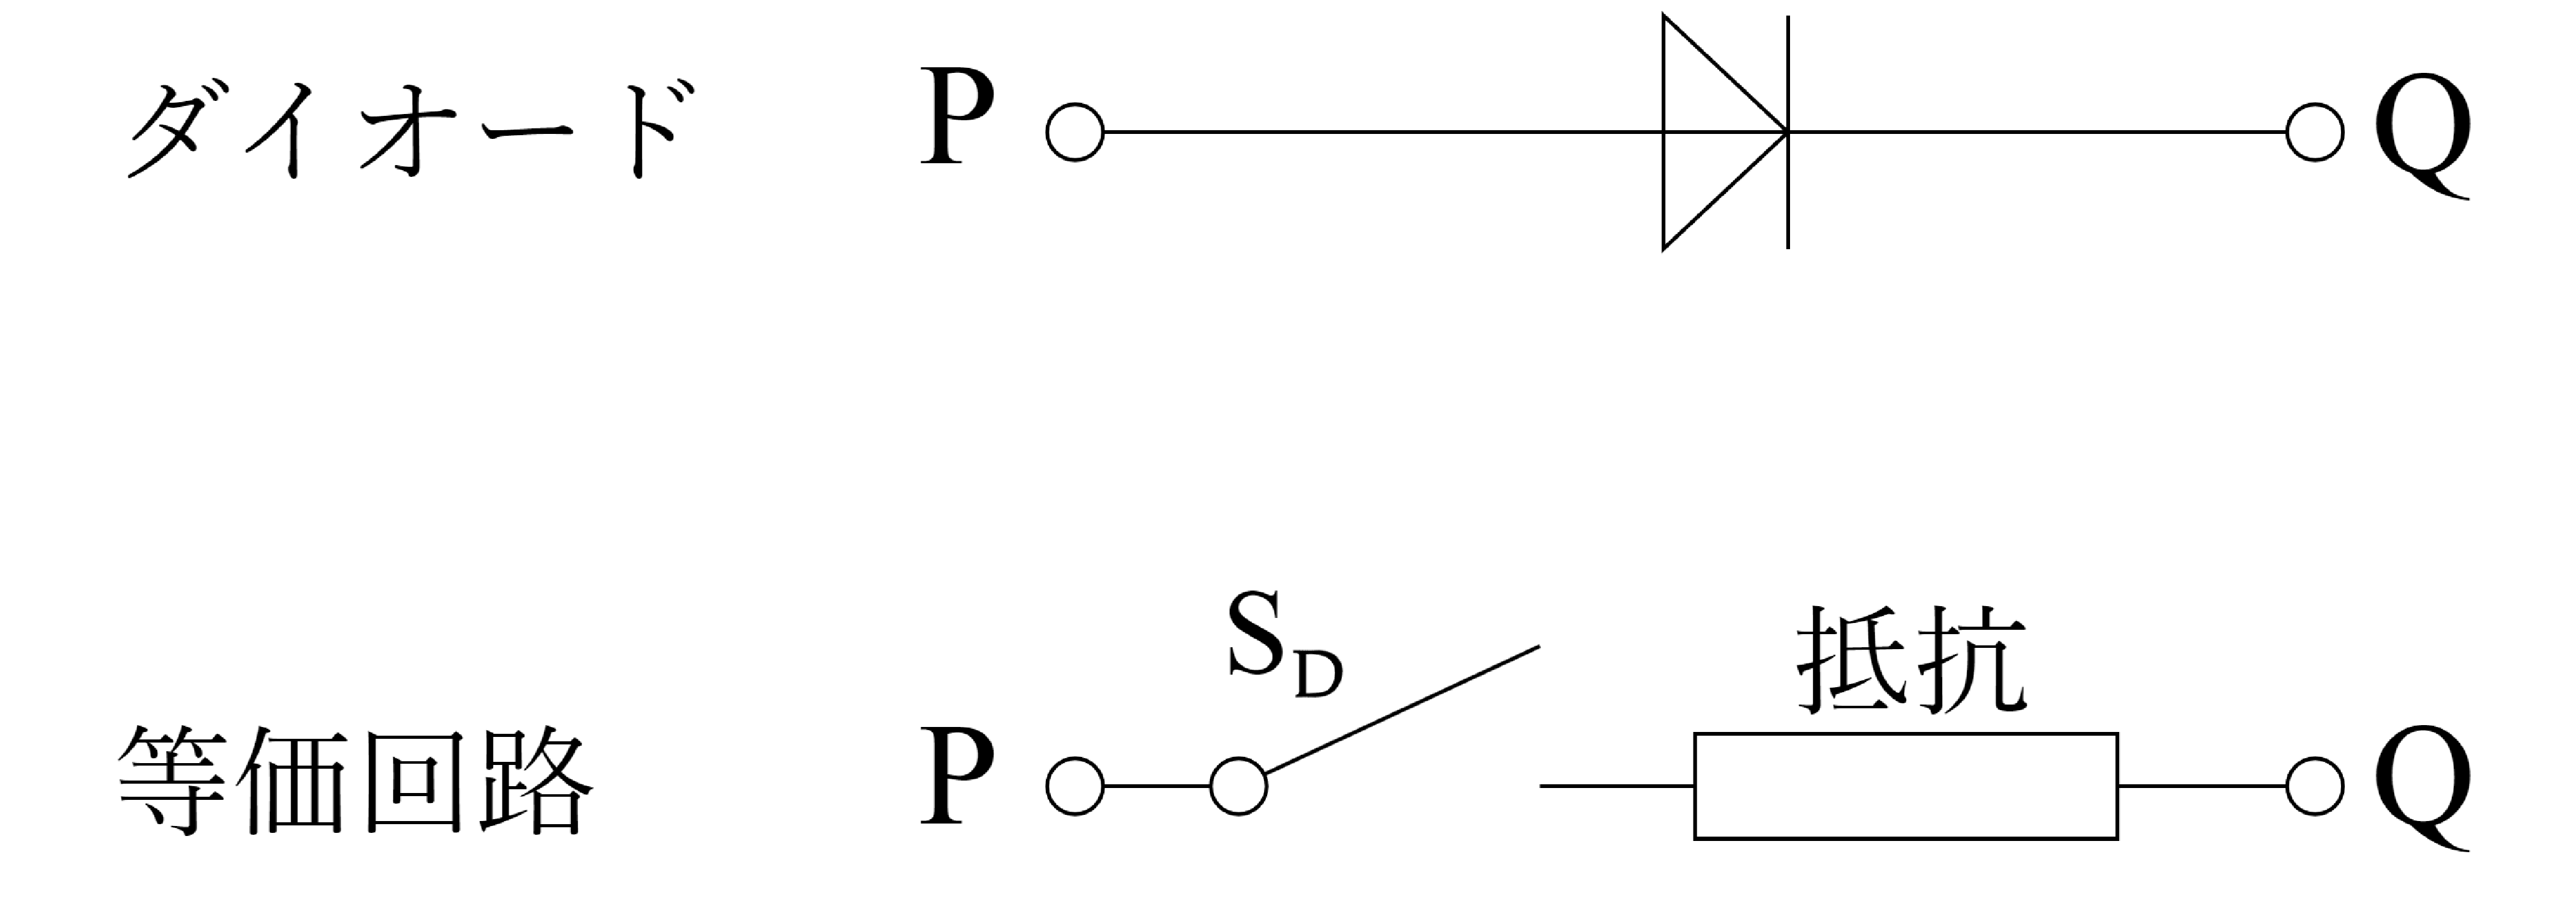
\includegraphics[width=6cm]{fig/fig_4_19_1.pdf}
    \caption{}
  \end{figure}
  \begin{figure}[H]
    \centering
    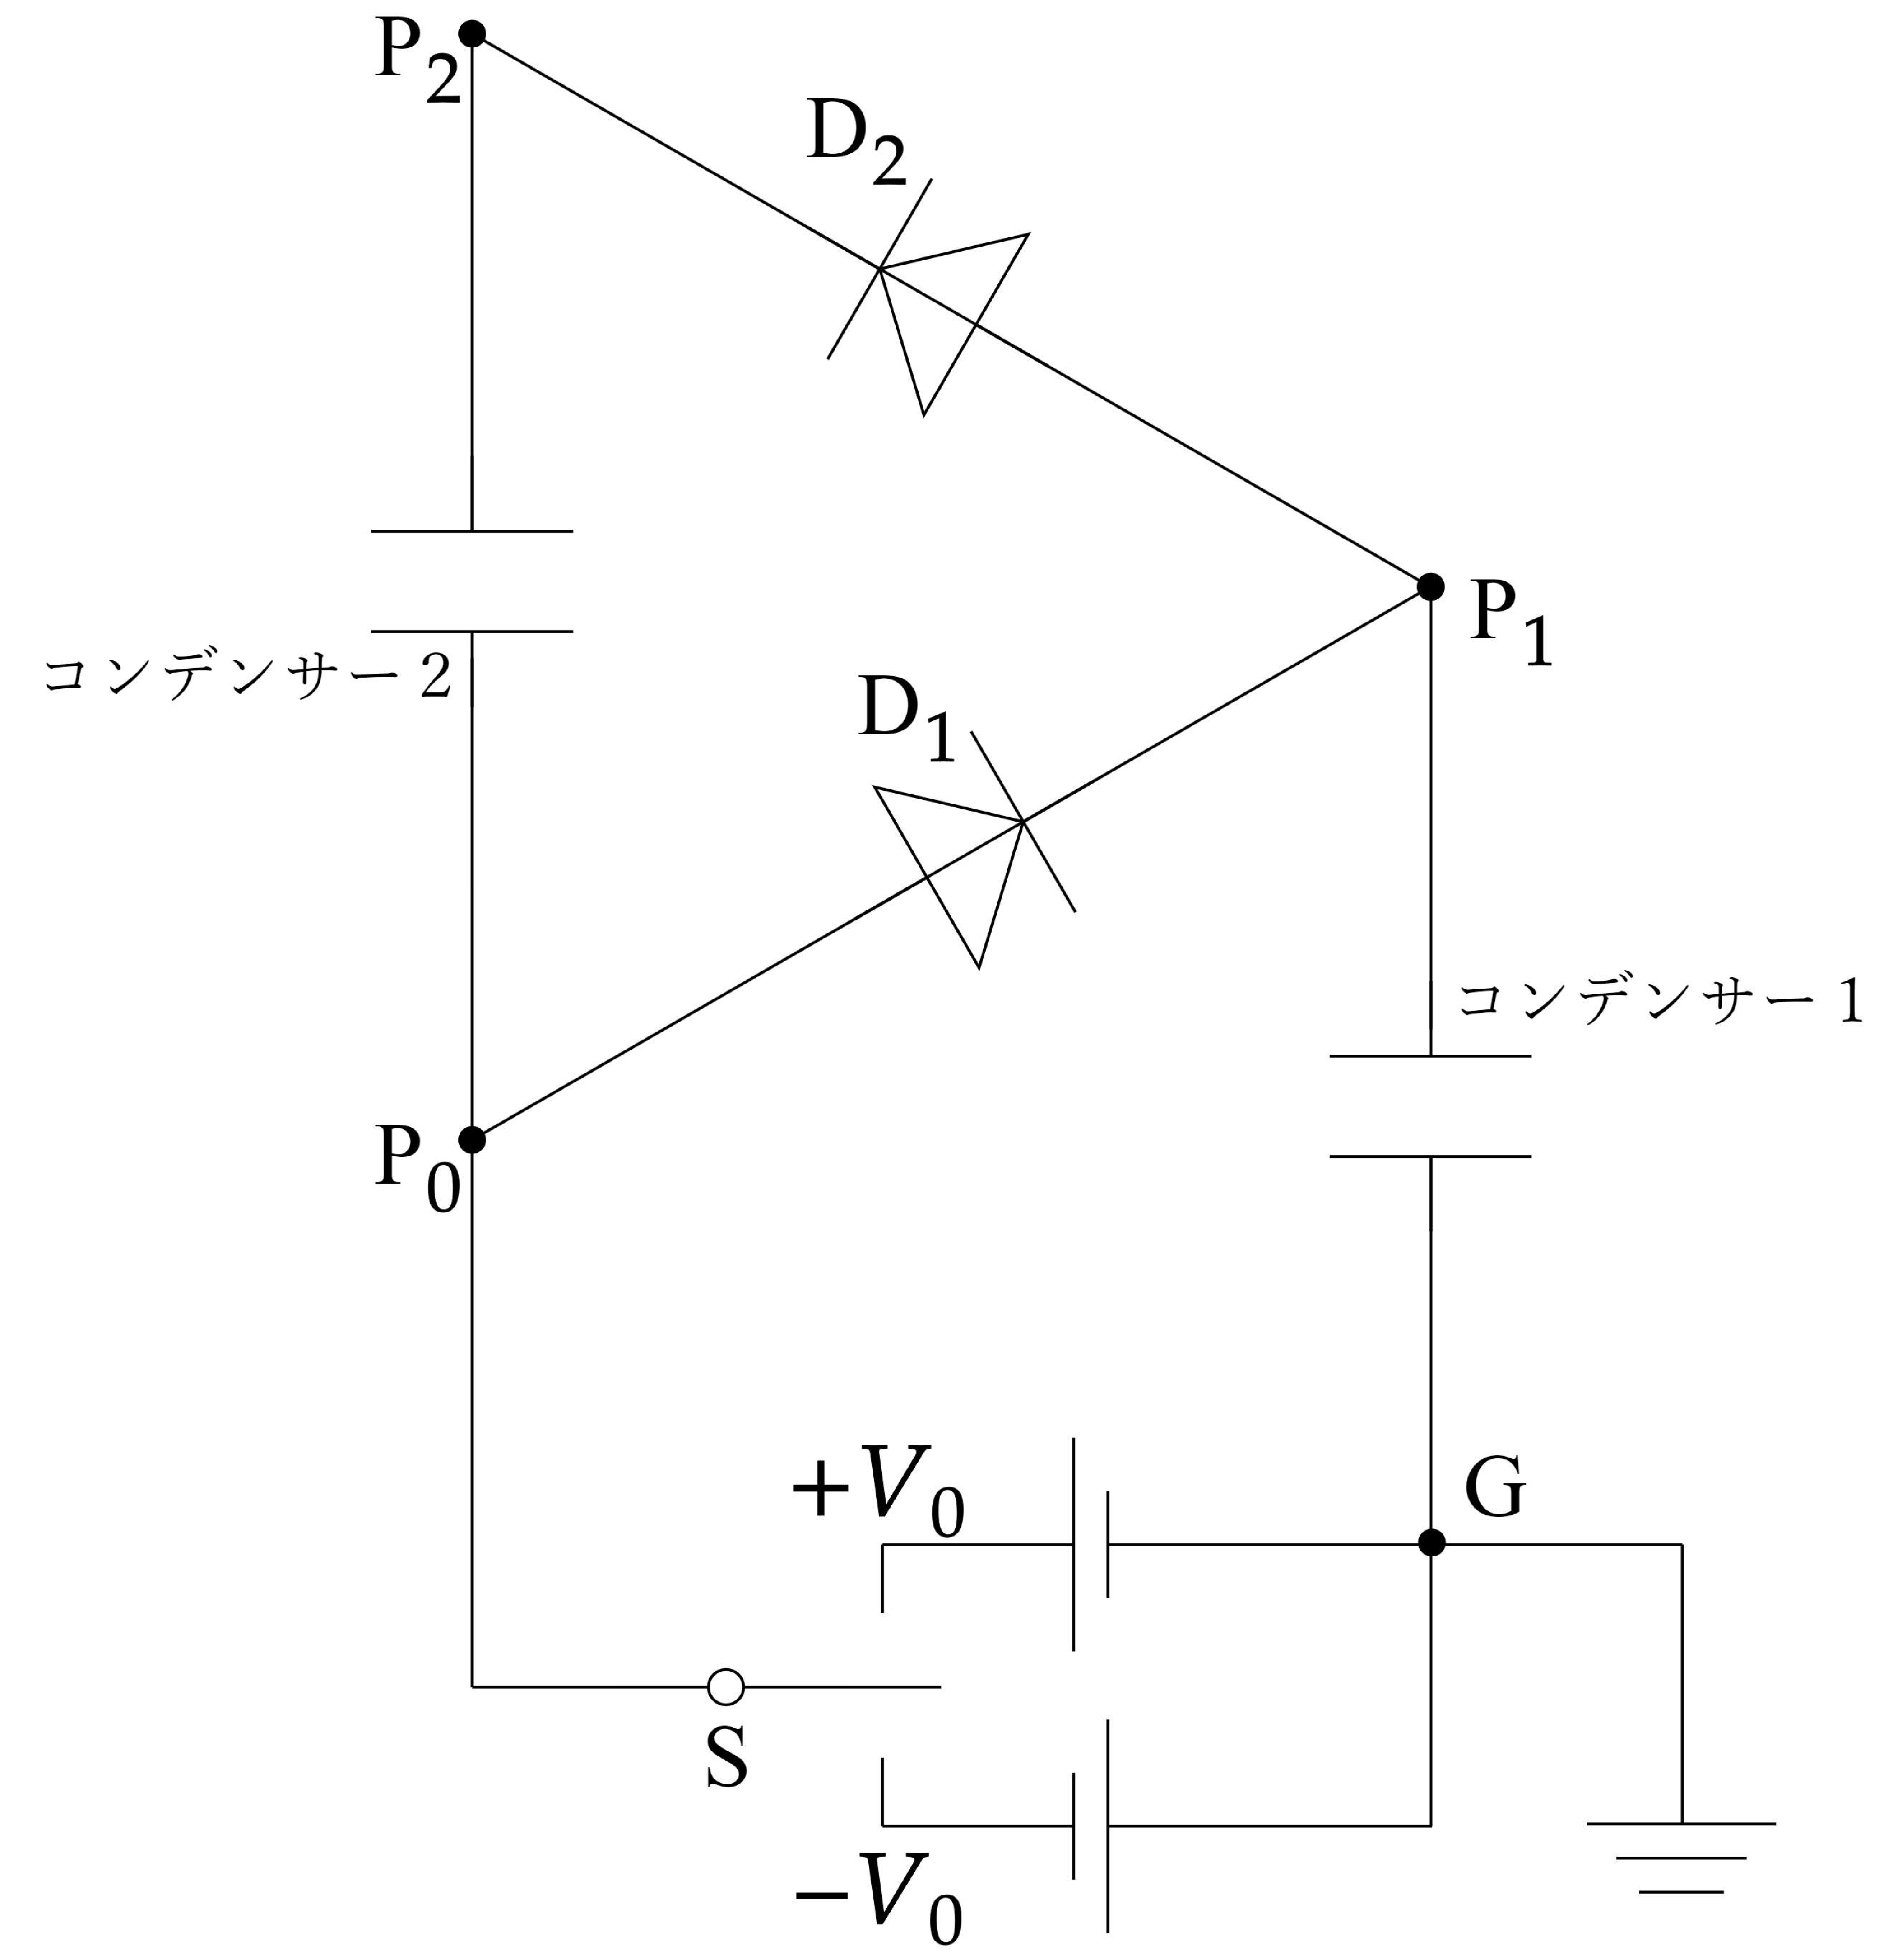
\includegraphics[width=6cm]{fig/fig_4_19_2.pdf}
    \caption{}
  \end{figure}
\end{minipage}
\begin{minipage}{0.4\linewidth}
  \centering
  \begin{figure}[H]
    \centering
    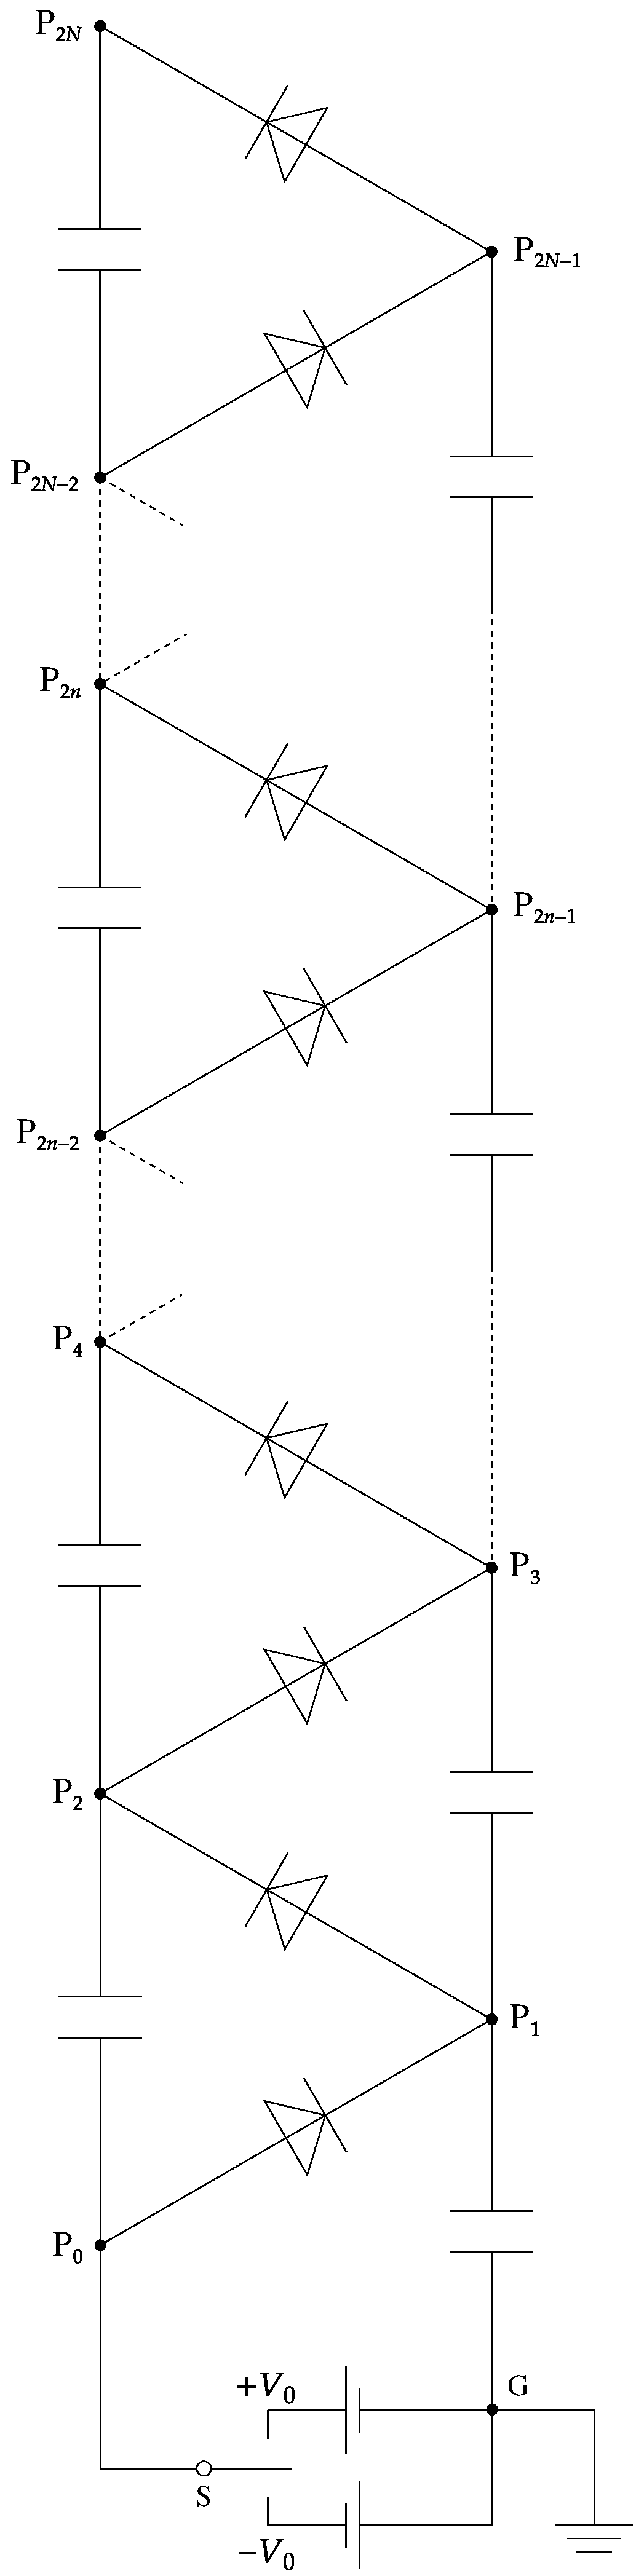
\includegraphics[width=5cm]{fig/fig_4_19_3.pdf}
    \caption{}
  \end{figure}
\end{minipage}


\end{document}
